\documentclass[12pt,x11names,a4paper]{article}
%Preamble

\usepackage{comment}
\usepackage[utf8]{inputenc}
\usepackage{amsmath}
\usepackage{amssymb}
\usepackage{amsthm}
\usepackage{enumitem}
\usepackage{mathrsfs}
\usepackage{mathtools}
\usepackage{esvect}
\usepackage{xfp}
\usepackage{xparse}
\usepackage{array}
\usepackage{changepage}
\usepackage{pdfpages}
\usepackage[parfill]{parskip}
\usepackage{anyfontsize}
\usepackage{alphalph}
\usepackage{ulem}
\usepackage{cancel}
\usepackage[framemethod=tikz]{mdframed}
\usepackage{xargs}
\usepackage{siunitx}              


\usepackage{algorithm}
\usepackage{algorithmic}
\usepackage{matlab-prettifier}
\usepackage{textcomp}
\usepackage{listings}
\usepackage[dvipsnames,svgnames]{xcolor}
\usepackage{colortbl}
\usepackage{eso-pic}
\usepackage[margin=1.35in]{geometry}
\usepackage{float}
\usepackage[danish]{babel}
\usepackage{tikz}
\usetikzlibrary{matrix,calc}
\usetikzlibrary{arrows}
\usetikzlibrary{arrows.meta}
\usetikzlibrary{decorations.pathreplacing}
\usetikzlibrary{decorations.pathreplacing,calligraphy}
\usetikzlibrary{patterns}
\usetikzlibrary{angles, quotes}
\usepackage{csquotes}
\usepackage{pdfpages}
\usepackage{fancyhdr}
\usepackage{lastpage}
\usepackage{pgfplots}
\usepackage{pgffor}

%Ændre følgende, hvis du vil have en anden bredde på pgfplots
\pgfplotsset{width=10cm,compat = 1.9}




\usepackage{caption}
\usepackage{subcaption}
\makeatletter
% \def\@seccntformat#1{%
%   \expandafter\ifx\csname c@#1\endcsname\c@section\else
%   \csname the#1\endcsname\quad
%   \fi}
 \makeatother
\counterwithin*{equation}{section}
\numberwithin{equation}{section}



%\newtheorem{setn}{Sætning}[section]
%\newtheorem{prop}[defn]{Proposition}
%\newtheorem{lem}[defn]{Lemma}
%\newtheorem{cor}[defn]{Korollar}

\newcommand\Tr{\textnormal{Tr}}
\newcommand\N{\textnormal{N}}
\newcommand{\suco}[2]{\left.#1\right|_{\mathbb{F}_{#2}}}
\renewcommand\qedsymbol{$\blacksquare$}
\theoremstyle{definition}
%\newtheorem{defn}[setn]{Definition}

\newcommand\Ker{\textnormal{Ker}\hspace{0.5mm}}
\renewcommand\Im{\textnormal{Im}\hspace{0.5mm}}
\newcommand\TS{\hspace{0.8mm}}

\usepackage{tcolorbox}
\tcbuselibrary{theorems}

\newmdtheoremenv[
	skipabove = 5pt,
	skipbelow = 5pt,
	roundcorner = 5,
	backgroundcolor = SeaGreen!30,
	linecolor = white, 
	]
	{defn}{ Definition }[section]

\newmdtheoremenv[
	skipabove = 5pt,
	skipbelow = 5pt,
	roundcorner = 5,
	backgroundcolor = RubineRed!20,
	linecolor = white, 
	]
	{setn}[defn]{ Sætning }
	

\newtheorem{eksempel}[defn]{Eksempel}

\newenvironment{exa}
	{\begin{eksempel}}
	{\unskip\hfill $\square$ \end{eksempel}}
\newtheorem{regel}[defn]{Regel}


\usepackage{graphicx}
\usepackage[backend=biber]{biblatex}
\addbibresource{biblio.bib}

\renewcommand{\mod}[1]{\ (\textnormal{mod }{#1})}
\usepackage{hyperref, bookmark}
\usepackage{booktabs}
\usepackage{calc}
\usepackage[nottoc,numbib]{tocbibind} 
\usepackage{multirow,bigdelim}

\renewcommand{\arraystretch}{1.3}
\newcommand\intd{\textnormal{d}}
\newcommand\e{\textnormal{e}}




\newenvironment{opgavetekst}[1]
{
	\begin{minipage}[t]{0.15\textwidth}
	 	\textbf{ #1}
	\end{minipage}
	\begin{minipage}[t]{0.85\textwidth}
		\rule{\textwidth}{0.3mm} \\
}
{ 
\\	\end{minipage}
}

\newenvironment{meretekst}
{
	\begin{minipage}[t]{0.15\textwidth}
	 	\phantom{h}
	\end{minipage}
	\begin{minipage}[t]{0.85\textwidth}
}
{ 
\\	\end{minipage}
}

\newenvironment{delopgave}[1]
{
	\begin{minipage}[t]{0.15\textwidth}
		\phantom{\textbf{Opgave}}		
		\textbf{\symbol{\numexpr96+ #1})}
	\end{minipage}
	\begin{minipage}[t]{0.85\textwidth}

	\begin{minipage}[t]{\textwidth}
}{
\end{minipage}
\phantom{h}\\
\end{minipage}
}


%\newcommand{opgavelinje}[1]{
%\begin{minipage}[t]{0.15\textwidth}
%\textbf{#1}
%\end{minipage} 
%\begin{minipage}[t]{\textwidth}
%\rule{0.81\textwidth}{0.3mm}
%\end{minipage}
%}





%Farver!
\definecolor{NorregGroen}{RGB}{0,105,78}





\newgeometry{margin=2cm}

\pagestyle{fancy}
\fancyhf{}

\rhead{Nørre Gymnasium\\1.w
}
\cfoot{Side \thepage \hspace{1pt} af \pageref{LastPage}}

%Husk at rette modul og dato!
\lhead{Aflevering 6\\ Matematik A  %<---------------------------------------RET
}
\chead{13. april 2026 %<----------------------------------------------------RET
}

\begin{document}

%
\includepdf[pages=-]{Forsider/aarsprove_1v.pdf}
\savegeometry{art}

\begin{titlepage}
\newgeometry{margin=0pt}

\begin{minipage}{0.27\textwidth}

\begin{tikzpicture}[overlay]
\fill[top color = NorregGroen!40, bottom color = NorregGroen] (6,10) rectangle (-10,-30);
\end{tikzpicture}
\end{minipage}
\begin{minipage}{0.73\textwidth}
\begin{center}
\phantom{h} \vspace{1cm}\\
\hspace{4cm}

\includegraphics[scale = 1]{Billeder/Norreg.png} \\
\phantom{h} \vspace{5cm}\\
\rule{0.7\textwidth}{0.3mm}\\
\phantom{h}\\
{\fontsize{50}{60}\selectfont Aflevering 6}\\%<---------------------------------------RET
\phantom{h}\\
\rule{0.7\textwidth}{0.3mm}\\
\Large 2026\\
\Large 1.w MA

\end{center}
\end{minipage}
\end{titlepage}
\loadgeometry{art}

%Udfyld afsnit herunder og lav til egen Latex-fil

%Kopier følgende til overskrift:

%\begin{center}
%\Huge
%Aflevering 1
%\end{center}
%\section*{Opgave 1}
%\stepcounter{section}
\begin{center}
%Opgavesætter er delt i to dele:\\
%Delprøve 1 kun med den centralt udmeldte formelsamling.\\
%Delprøve 2 med alle hjælpemidler.
\end{center}

\section*{Krav til formidling af din besvarelse}

Ved bedømmelse af helhedsindtrykket af besvarelsen af de enkelte opgaver lægges særlig vægt på følgende fire punkter:
\begin{itemize}
\item[$\cdot$] \textbf{Redegørelse og dokumentation for metode} \\
Besvarelsen skal indeholde en redegørelse for den anvendte løsningsstragegi med dokumentation i form af et passende antal mellemregninger \textit{eller} matematiske forklaringer på metoden, når et matematisk værktøjsprogram anvendes.
\item[$\cdot$] \textbf{Figurer, grafer og andre illustrationer} \\
Besvarelsen skal indeholde hensigtsmæssig brug af figurer, grafer og andre illustrationer, og der skal være tydelige henvisninger til brug af disse i den forklarende tekst.
\item[$\cdot$] \textbf{Notation og layout}\\
Besvarelsen skal i overensstemmelse med god matematisk skik opstilles med hensigtsmæssig brug af symbolsprog, og med en redegørelse for den matematiske notation, der indføres og anvendes, og som ikke kan henføres stil standardviden.
\item[$\cdot$] \textbf{Formidling og forklaring}\\
Besvarelsen af rene matematikopgaver skal indeholde en angivelse af givne oplysninger og korte forklaringer knyttet til den anvendte løsningsstrategi beskrevet med brug af almindelig matematisk notation. 

Besvarelsen af opgaver, der omhandler matematiske modeller, skal indeholde en kort præsentation af modellens kontekst, herunder betydning af modellens parametre. De enkelte delspørgsmål skal afsluttes med en præcis konklusion præsenteret i et klart sprog i relation til konteksten.
\end{itemize}

\newpage

\begin{center}
	\LARGE
	Med hjælpemidler
\end{center}
\begin{opgavetekst}{Opgave 1}
	To linjer $l$ og $m$ er givet ved henholdsvis
	\begin{align*}
		l: \ 5x + 19y &= 12, \\
		m: \ 10x -10y &= 29.
	\end{align*}
\end{opgavetekst}
\begin{delopgave}{1}
	Orientér dig i Maple-filen \textit{To ligninger med to ubekendte} under forløbet \textit{Ligninger} på Teams og bestem derefter 
	skæringspunktet mellem $l$ og $m$. 
\end{delopgave}
\begin{delopgave}{2}
	Bestem løsningen til ligningssystemet
	\begin{align*}
		x + 2y + 3z &= 10,\\
		10x -5y + 3z &= 8, \\
		-2x + 9y -11z &= -3.
	\end{align*}
\end{delopgave}
\begin{opgavetekst}{Opgave 2}
	To polynomier $p$ og $q$ er givet ved
	\begin{align*}
		p(x) &= -2x^3 + 14x^2 + 8x - 100,\\
		q(x) &= -5x^3 - 13x^2 -10x + 68. 
	\end{align*}
\end{opgavetekst}
\begin{delopgave}{1}
	Orientér dig i Maple-filen \textit{Graftegning i Maple} under \textit{Vækst} på Teams og tegn graferne for $p$ og $q$ for $x \in [-8,3]$.
\end{delopgave}
\begin{delopgave}{2}
	Bestem koordinatsættet til skæringspunkterne for graferne til $p$ og $q$, og sammenlign dit resultat med 
	tegningen af graferne. 
\end{delopgave}

\newpage

\begin{opgavetekst}{Opgave 3}
	En funktion $f$ er givet ved
	\begin{align*}
		f(x) = b \cdot a^x
	\end{align*}
	og opfylder, at $f(2) = 5$ samt $f(4) = 12$
\end{opgavetekst}
\begin{delopgave}{1}
	Bestem tallene $b$ og $a$. 
\end{delopgave}
\begin{meretekst}
	En anden funktion $g$ er givet ved
	\begin{align*}
		g(x) = 1.2 \cdot x^d 
	\end{align*}
	og opfylder også, at $g(2) = 5$. 
\end{meretekst}
\begin{delopgave}{2}
	Bestem tallet $d$ og tegn grafen for $g$. 
\end{delopgave}
\begin{delopgave}{2}
	Orientér dig i Maple-filen \textit{Ligningsløsning på interval} under forløbet \textit{Ligninger} og bestem det andet skæringspunkt
	 mellem $f$ og $g$. 
\end{delopgave}

\begin{opgavetekst}{Opgave 4}
	\begin{center}
		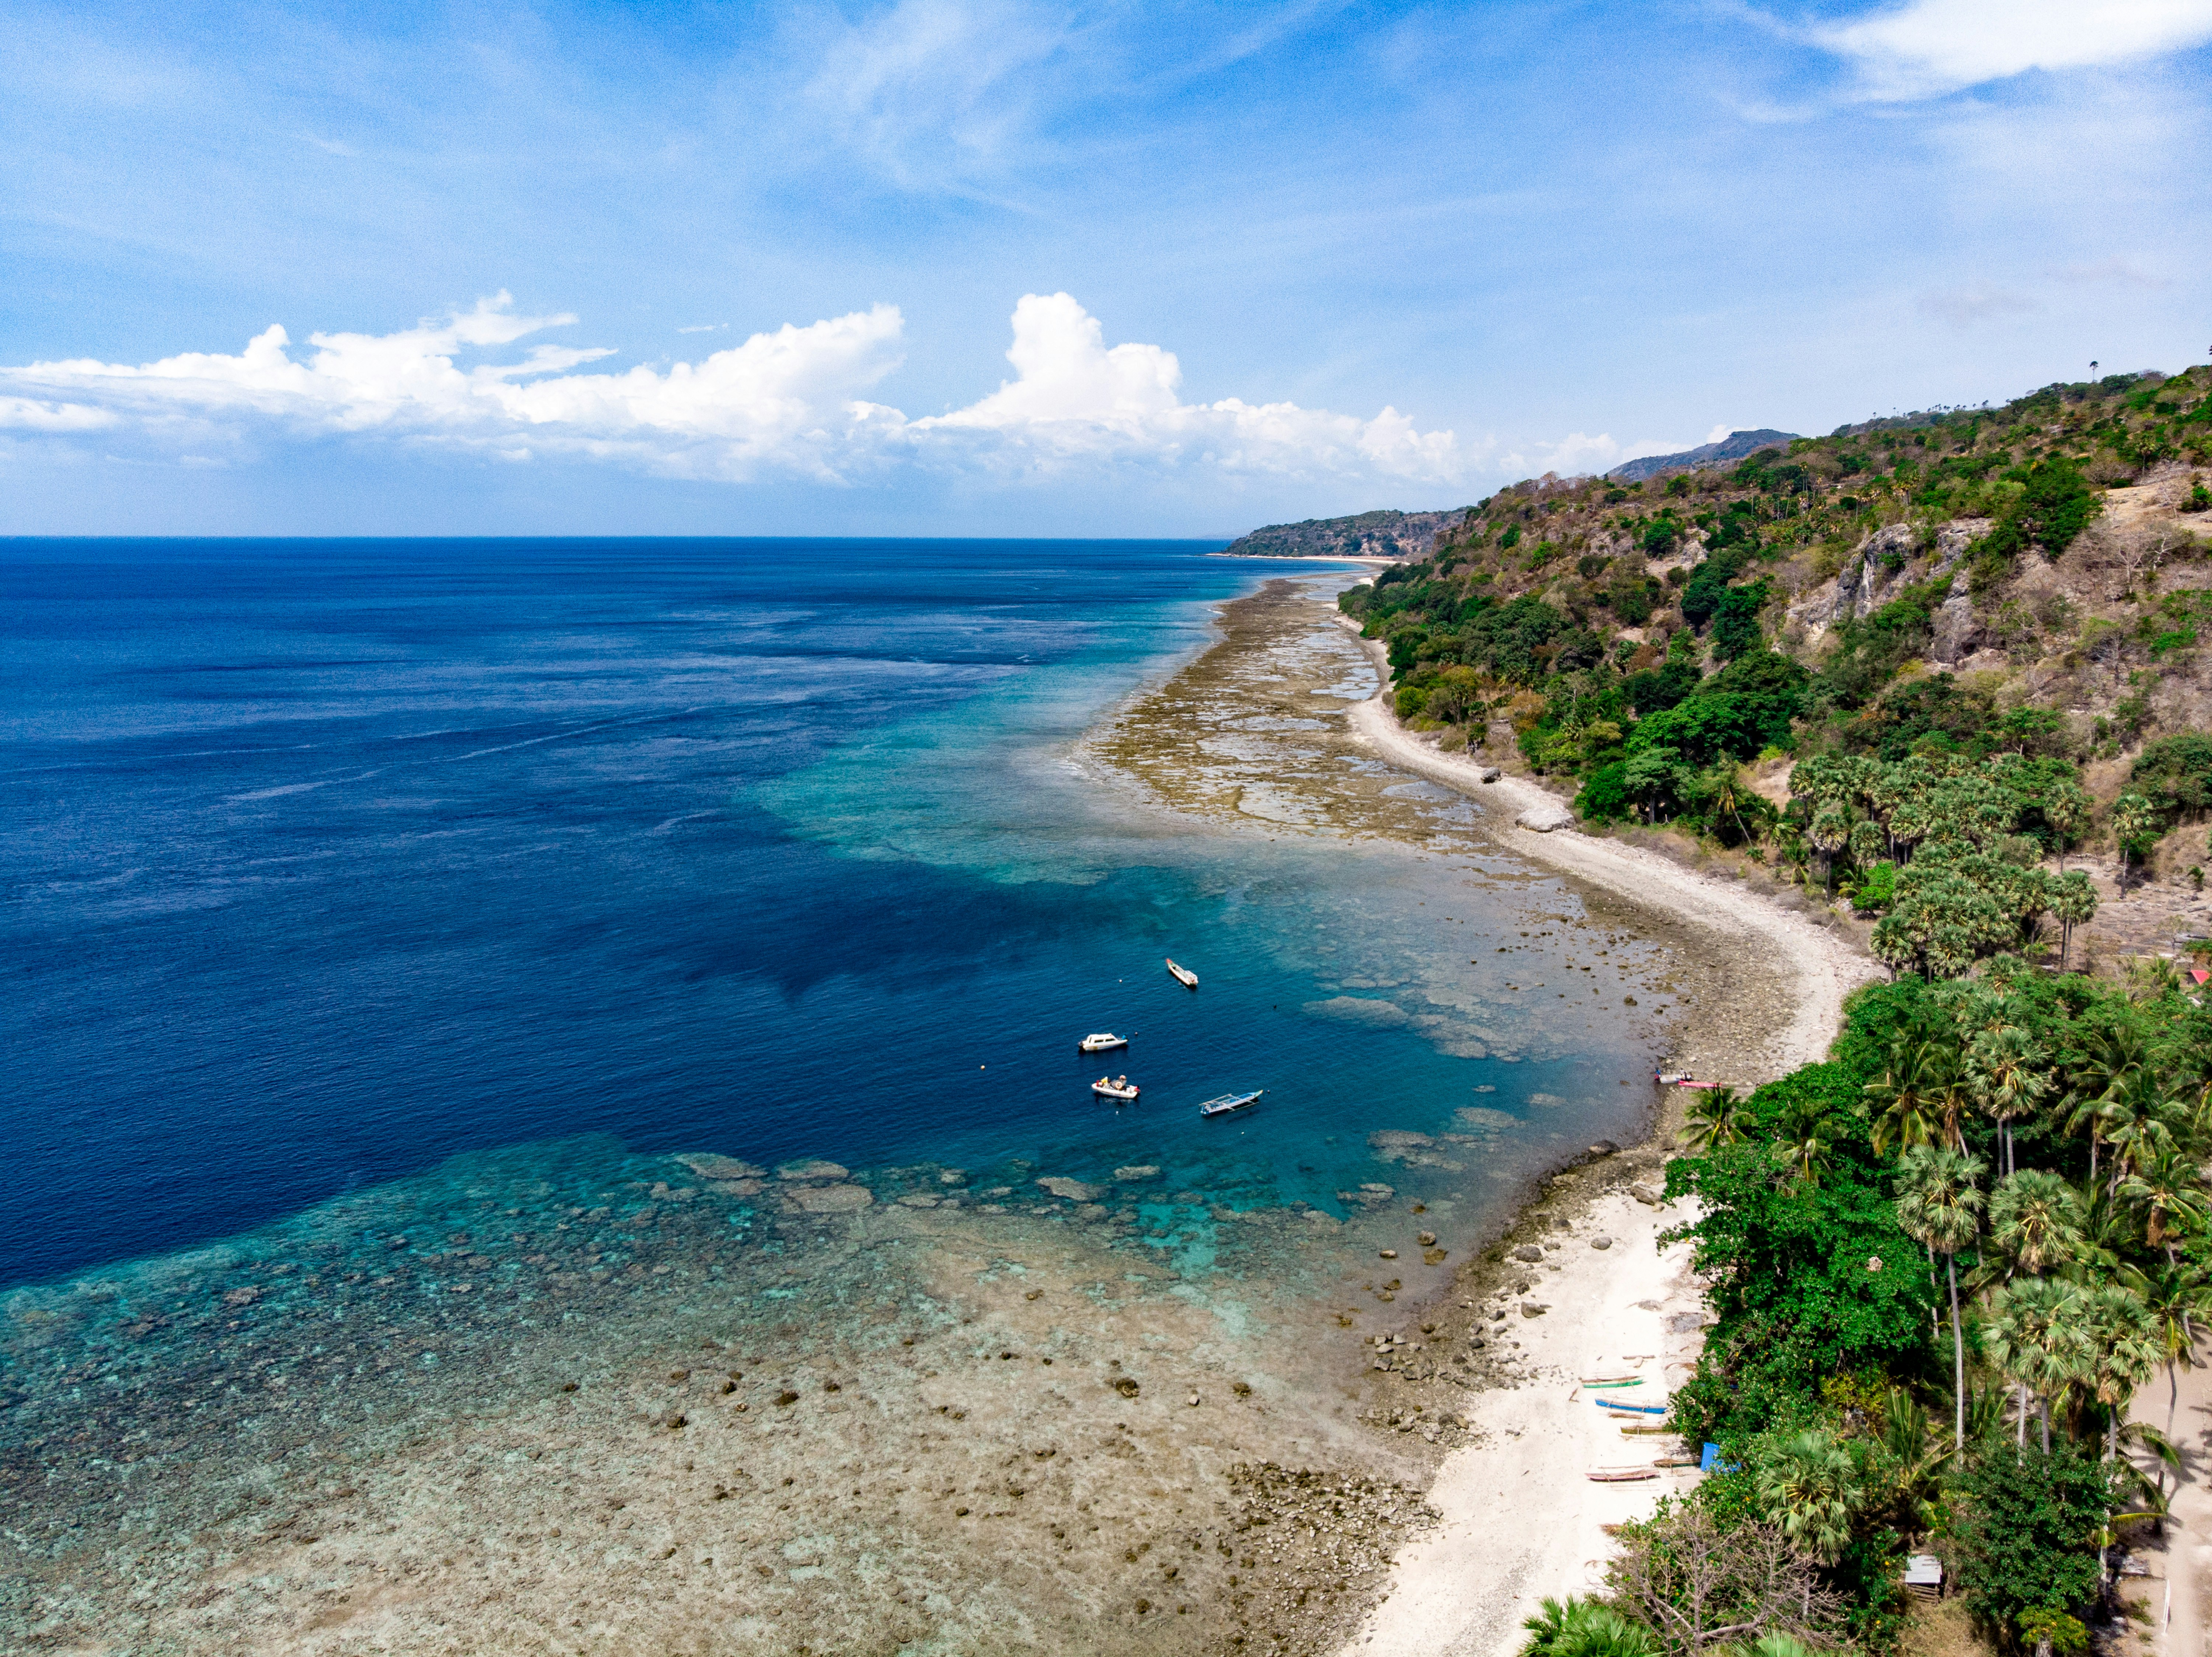
\includegraphics[width = 0.6\textwidth]{Billeder/oesttimor}
	\end{center}
	Bruttonationalproduktet i tidsperioden 1998-2023 for den tidligere portugisiske koloni Østtimor fremgår af \href{https://github.com/ChristianJLex/TeachingNotes/raw/master/2024-2025/Data%20og%20lign/BNPoesttimor.xlsx}{\color{blue!60}dette datasæt.}
	Det formodes, at den forløbne tid efter 1998 $t$ og BNP i Østtimor $f$ (i mia. USD) kan beskrives ved en sammenhæng af
	typen
	\begin{align*}
		f(t) = b\cdot a^t
	\end{align*}	 
\end{opgavetekst}
\begin{delopgave}{1}
	Orientér dig i filen \textit{Ændring af årstal} under \textit{Vækst} på Teams og bestem tallene $b$ og $a$.
\end{delopgave}
\begin{delopgave}{2}
	Giv en fortolkning af tallene $a$ og $b$. 
\end{delopgave}
\begin{delopgave}{3}
	Bestem det årstal, hvor Østtimor vil have et BNP på 40 mia ifølge modellen. 
\end{delopgave}
\newpage

\begin{opgavetekst}{Opgave 5}
	Et polynomium $p$ er givet ved
	\begin{align*}
		p(x) = 7x^5+2x^3-10x^2+5x+12
	\end{align*}
\end{opgavetekst}
\begin{delopgave}{1}
	Orientér dig i filen \textit{Rødder for polynomier} under \textit{Polynomier} på Teams og bestem rødderne for $p$.
\end{delopgave}
\end{document}




